\documentclass[conference]{IEEEtran}
\ifCLASSINFOpdf
\usepackage[pdftex]{graphicx}
\else
\fi
\usepackage{hyperref}
\hypersetup{
    colorlinks=true,
    linkcolor=blue,
    filecolor=magenta,      
    urlcolor=blue,
}

\urlstyle{same}
% correct bad hyphenation here
\hyphenation{op-tical net-works semi-conduc-tor}
\usepackage{amsmath}
\usepackage[section]{placeins}
\usepackage[font=footnotesize]{caption}
\usepackage{float}

\begin{document}
\title{Movies' IMDb Rating Prediction}
\author{\IEEEauthorblockN{Advait Lonkar}
\IEEEauthorblockA{IMT2017002\\International Institute of Information\\ Technology, Bangalore}
\and
\IEEEauthorblockN{Gandharv Suri}
\IEEEauthorblockA{IMT2017017\\International Institute of Information\\ Technology, Bangalore}
\and
\IEEEauthorblockN{Mili Goyal}
\IEEEauthorblockA{IMT2017513\\International Institute of Information\\ Technology, Bangalore}
}
\maketitle
\begin{abstract}
One simple, but an effective way to determine if a movie is worth watching is to use its IMDb rating. The IMDb top 250 list is, despite the subjective nature of the matter, the list of best movies one can watch. We present a machine learning model to predict the IMDb rating of a movie based on various features provided in the dataset.

\textit{Keywords : IMDb rating, numerical features, }
\end{abstract}
\section{Introduction}
IMDb (Internet Movie Database) is an online database of information related to films, television programs, home videos, video games, and streaming content online – including cast, production crew and personal biographies, plot summaries, trivia, fan and critical reviews, and ratings \cite{IMDB}.\\
IMDb registered users can cast a vote (from 1 to 10) on every released title in the database. Individual votes are then aggregated and summarized as a single IMDb rating, visible on the title’s main page \cite{rating}.\\
The IMDb ratings are accurately calculated using a consistent, unbiased formula, but by no means are these ratings qualitatively \textit{accurate}. An argument can be made that the ratings are too simplistic, which is quite fair : millions of users rate an artistic expression and reduce it into a range of 1 to 10, so obviously some of the nuances of what makes a movie good are lost. \\
But more often than not, people visit IMDb to rate the latest movie they had watched, check ratings of other movies, make watch lists accordingly, and many other such activities. Though the rating is only a number, it can be very informative and useful in itself. A rating cast by thousands of viewers generally represents a well-aggregated rating of a movie. \\
The goal of the project is to predict the IMDb rating of a movie provided various features in the dataset.\\
\section{Problem Statement}
Given various data-points of a movie, predict where the IMDb rating of the movie falls in the range of 1 to 10.\\
This problem falls under the domain of \textbf{Classification}, since we are going to predict the range in which the rating is going to fall and not the exact rating of the movie.\\
The evaluation metrics of the presented model will be the variance, standard deviation, root-mean-square-error of the predicted IMDb ratings v/s the actual IMDb rating of a particular movie.\\
\newpage
\section{Data}
\subsection{Data Description}
We have a dataset of 5,043 samples which will later be split into training and testing sets. The dataset was taken from Kaggle \cite{data}.\\
The dataset consists of the following fields:
\begin{itemize}
	\item \textbf{color} : a string field which identifies the color of the movie, color or black and white.
	\item \textbf{director$\_$name} : a string field which identifies the director of the movie.
	\item \textbf{num$\_$critic$\_$for$\_$reviews} : a numeric field which identifies the number of critic reviewers of a movie.
	\item \textbf{duration} : a numeric field which identifies the duration of the movie.
	\item \textbf{director$\_$facebook$\_$likes} : a numeric field which identifies the number of likes on facebook for the director of the movie.
	\item \textbf{actor$\_$3$\_$facebook$\_$likes} : a numeric field which identifies the number of likes on facebook of the 3rd actor of the movie.
	\item \textbf{actor$\_$2$\_$name} : a string field which identifies the name of the 2nd actor of the movie.
	\item \textbf{actor$\_$1$\_$facebook$\_$likes} : a numeric field which identifies the number of likes on facebook of the 1st actor of the movie.
	\item \textbf{gross} : a numeric field which identifies the gross revenue of the movie. 
	\item \textbf{genres}  : a string field which identifies the genre of the movie. 
	\item \textbf{actor$\_$1$\_$name} : a string field which identifies the name of the 1st actor of the movie.
	\item \textbf{movie$\_$title} : a string field which identifies the title of the movie.
	\item \textbf{num$\_$voted$\_$users} : a numeric field which identifies the number of users who voted for the movie. 
	\item \textbf{cast$\_$total$\_$facebook$\_$likes} : a numeric field which identifies the number of likes on facebook of the cast of the movie.
	\item \textbf{actor$\_$3$\_$name} : a string field which identifies the name of the 3rd actor of the movie.
	\item \textbf{facenumber$\_$in$\_$poster} : a numeric field which identifies the number of faces in the poster of the movie.
	\item \textbf{plot$\_$keywords}  : a string field which identifies the plot keywords of the movie.
	\item \textbf{movie$\_$imdb$\_$link} : a string field which identifies the imdb link of the movie. 
	\item \textbf{num$\_$user$\_$for$\_$reviews} : a numeric field which identifies the number of user for reviews of the movie. 
	\item \textbf{language}  : a string field which identifies the language of the movie.
	\item \textbf{country}  : a string field which identifies the country of the movie.
	\item \textbf{content$\_$rating} : a string field which identifies the conten rating (R or PG-13) of the movie.
	\item \textbf{budget} : a numeric field which identifies the budget of the movie.
	\item \textbf{title$\_$year} : a numeric field which identifies the year of release of the movie. 
	\item \textbf{actor$\_$2$\_$facebook$\_$likes} : a numeric field which identifies the number of likes on facebook of the 2nd actor of the movie.
	\item \textbf{imdb$\_$score} : a numeric field which identifies the imdb score of the movie.
	\item \textbf{aspect$\_$ratio}  : a numeric field which identifies the aspect ratio of the movie. 
	\item \textbf{movie$\_$facebook$\_$likes}  : a numeric field which identifies the number of likes on facebook of the movie.\\
\end{itemize}
\subsection{Data Exploration and Visualization}
In this section, we explore the dataset through various types of plots -
% IMBD-score histogram
\begin{figure}[H]
  \centering	
  \captionsetup{justification=centering}
  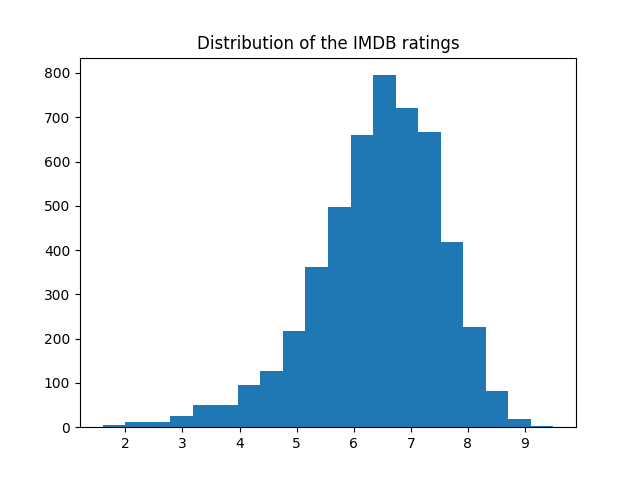
\includegraphics[height=8cm, width=9cm, trim={20mm 0mm 10mm 0mm},clip]{../visualizations/IMDB-Score-Histogram}
  \caption{IMDB-Score histogram}
  \label{fig:fig1}
\end{figure}
Fig. 1 shows the distribution of IMDb scores with buckets of size 200. We can observe that a majority of movies have a rating between 5.5 and 7.5.

% Language histogram
\begin{figure}[H]
  \centering	
  \captionsetup{justification=centering}
  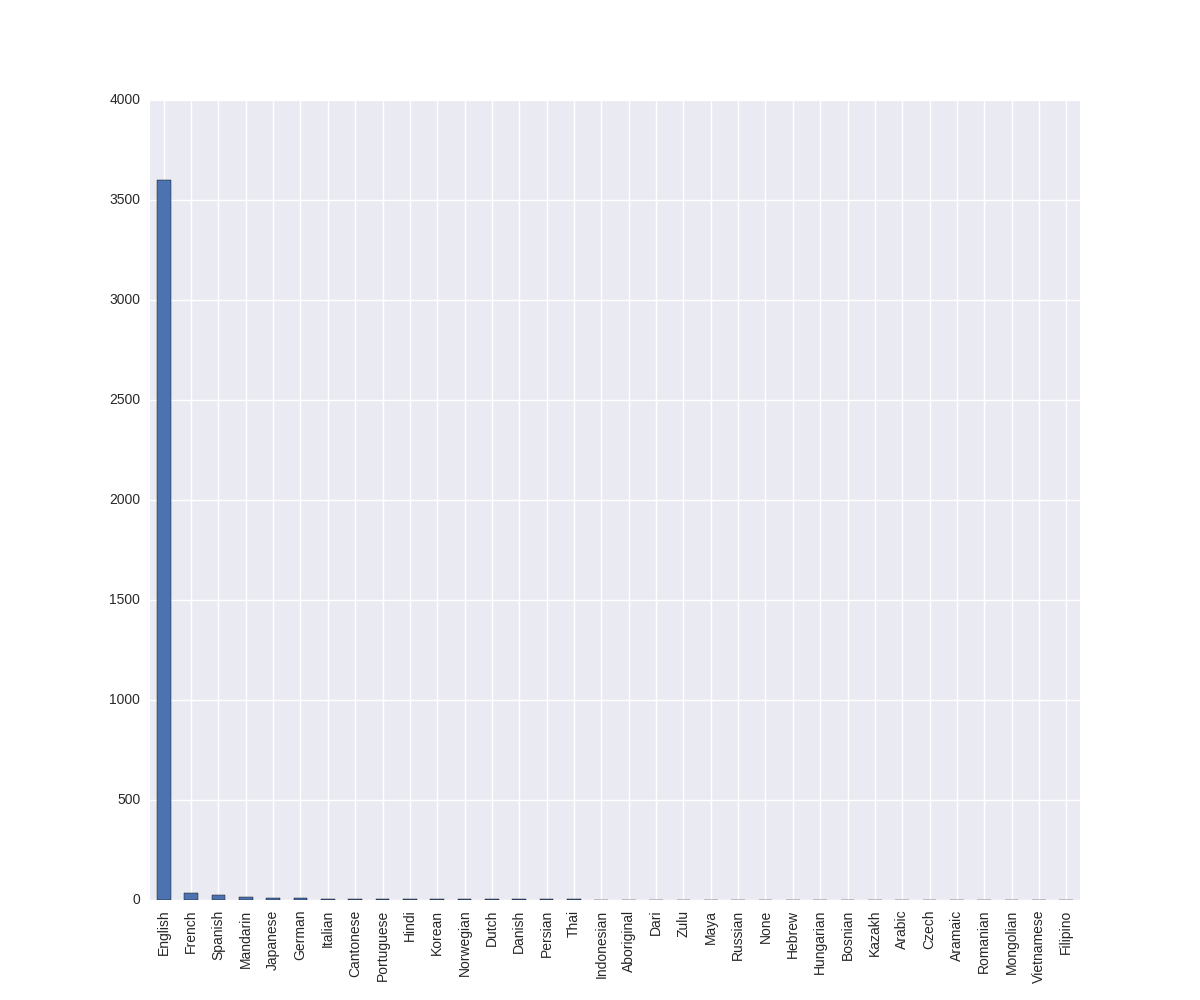
\includegraphics[height=8cm, width=10cm, trim={20mm 0mm 10mm 20mm},clip]{../visualizations/Language-Histogram}
  \caption{Language frequency plot}
  \label{fig:fig2}
\end{figure}
Fig. 2 shows the distribution of movies according to the language in which they were made. We can observe that an overwhelming majority of the movies are in English language and the rest of the movies are made in all the other languages.

% Country histogram
\begin{figure}[H]
  \centering	
  \captionsetup{justification=centering}
  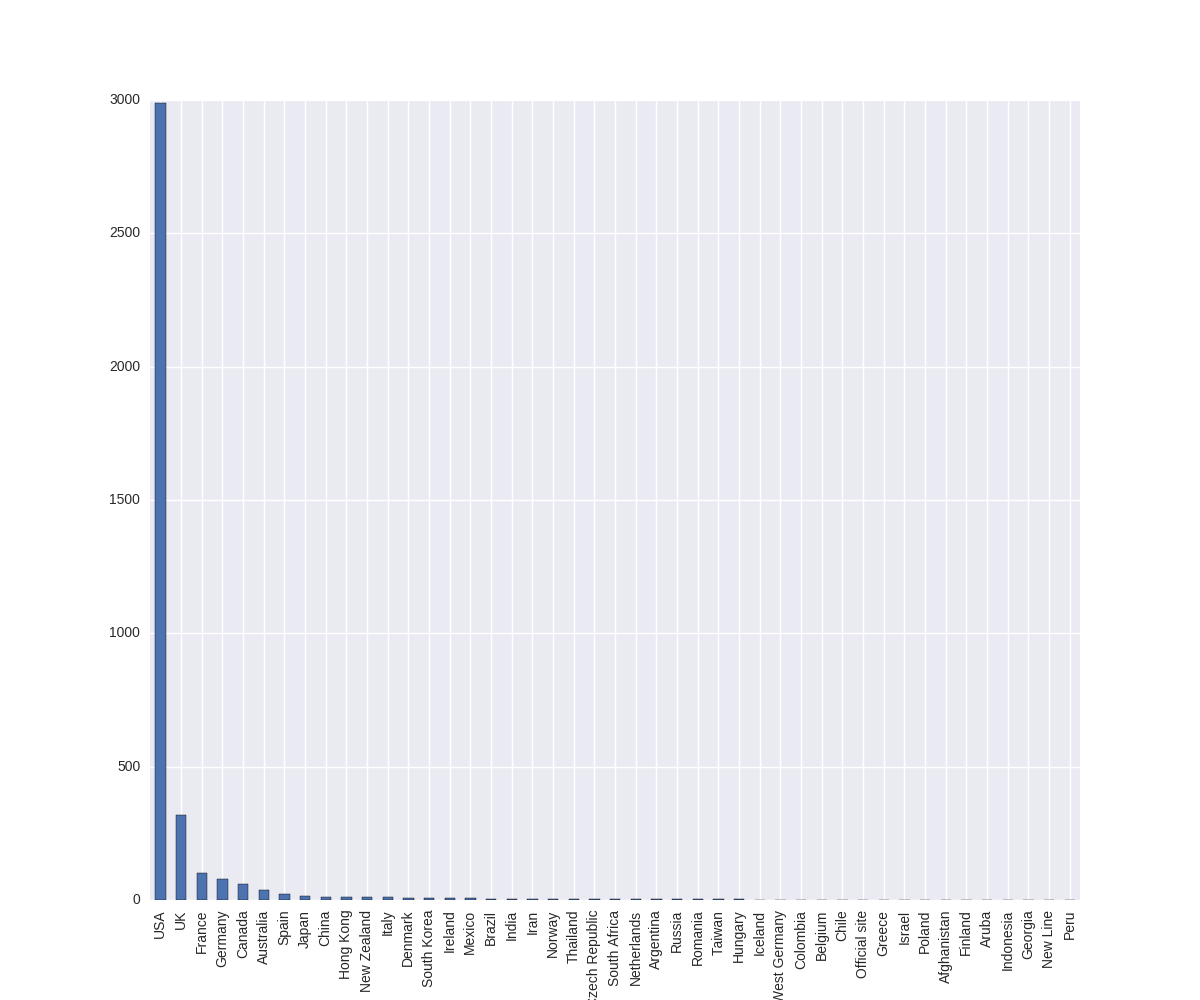
\includegraphics[height=8cm, width=10cm, trim={20mm 0mm 10mm 20mm},clip]{../visualizations/Country-Histogram.png}
  \caption{Country frequency plot}
  \label{fig:fig3}
\end{figure}
Fig. 3 shows the distribution of movies according to the countries in which they were made. We can observe that an overwhelming majority of the movies are from the USA. UK also has a fair share of movies. All  the other countries make up for the rest of the data.

% Color histogram
\begin{figure}[H]
  \centering	
  \captionsetup{justification=centering}
  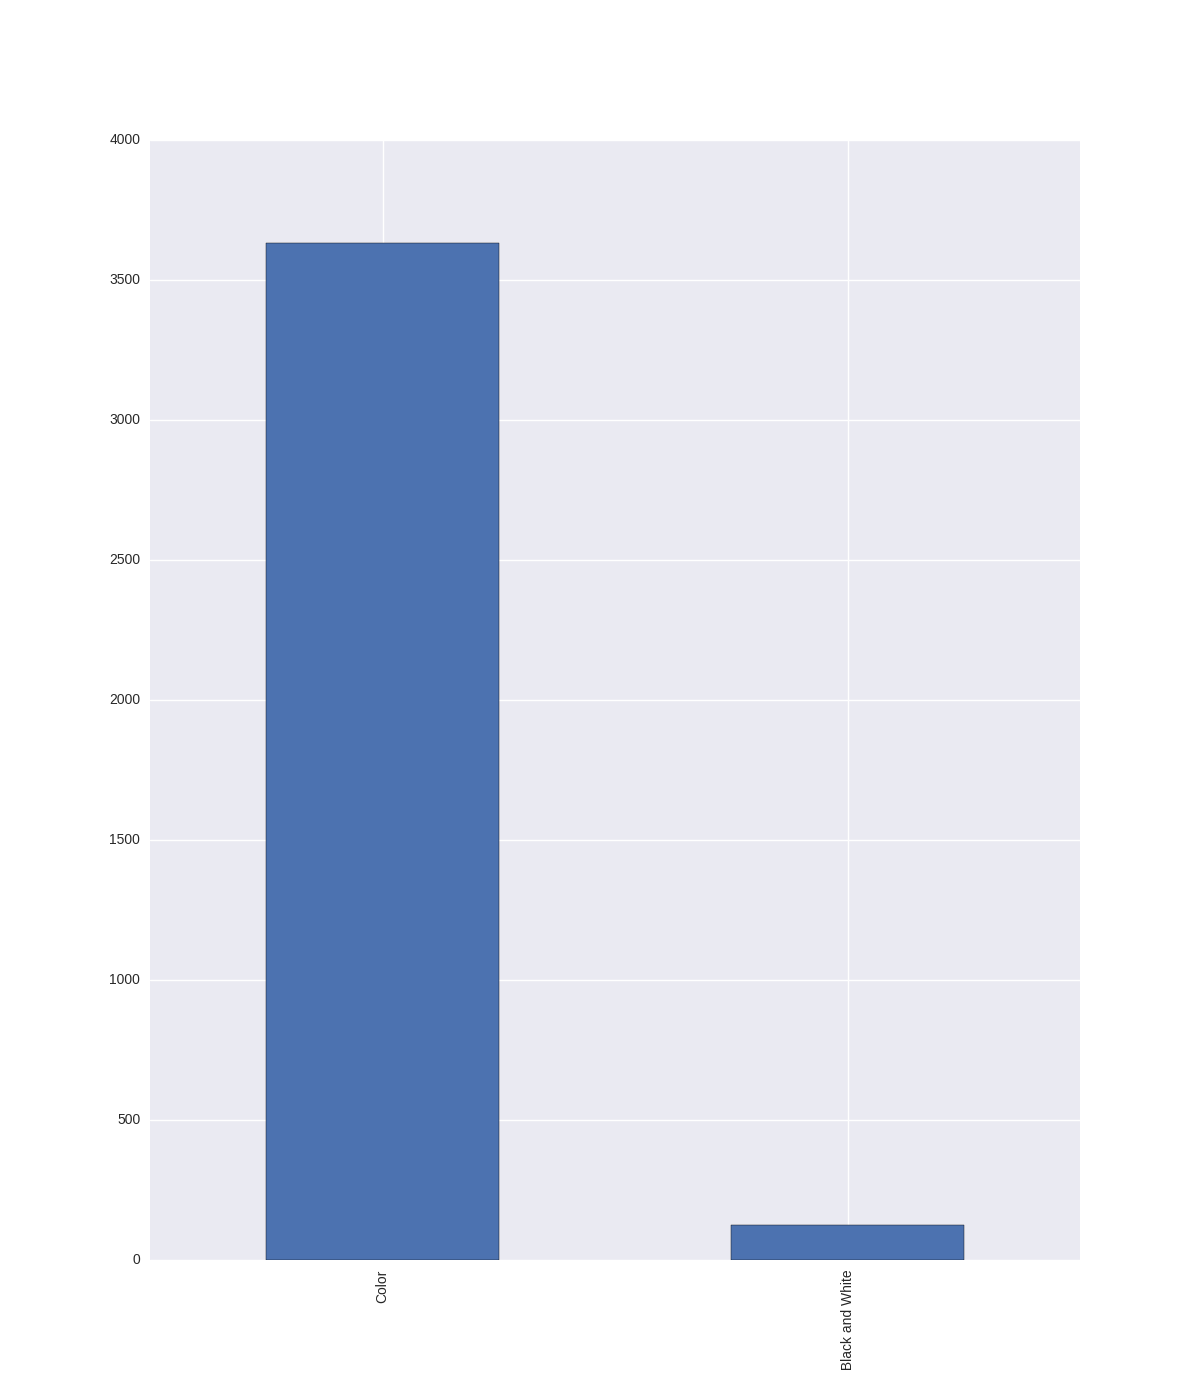
\includegraphics[height=8cm, width=9cm, trim={30mm 0mm 20mm 0mm},clip]{../visualizations/Colour-Histogram}
  \caption{Color frequency plot}
  \label{fig:fig4}
\end{figure}
Fig. 4 shows that the majority of the movies are colored while very few are black-and-white.

% Correlation matrix
\begin{figure}[H]
  \centering	
  \captionsetup{justification=centering}
  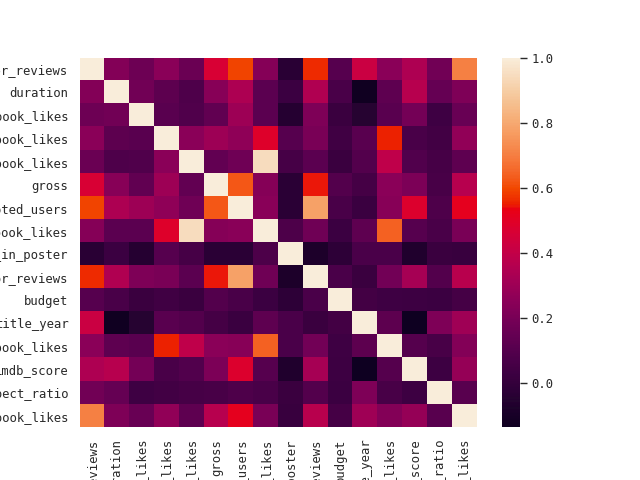
\includegraphics[height=8.5cm, width=10cm, trim={20mm 20mm 20mm 40mm},clip]{../visualizations/corr_matrix.png}
  \caption{Correlation matrix among all the features.}
  \label{fig:fig5}
\end{figure}
Fig. 5 shows the correlation matrix among the features. The covariance values of all the features are investigated against the IMDb score.

\newpage
\section{Pre-Processing}
\subsection{Dropping rows}
The columns $gross$ and $budget$ had the maximum number of missing values, 884 and 492 respectively. Imputation of so many values would provide faulty results, so we decided to drop the rows corressponding to the missing fields of columns $gross$ and $budget$.\\

\subsection{Dropping columns}
	\begin{enumerate}
		\item $aspect\_ratio$ : The two most frequent values of $aspect\_ratio			$ and the rest of the $aspect\_ratio$ values had similar mean IMDb 				ratings, i.e. the aspect ratio values did not have any significant effect on the IMDb ratings. So we dropped the column $aspect\_ratio$.\\
		
		\item $language$ : Most of the movies (more than 90$\%$) are in 				English, so we dropped the column $language$.\\
		
		\item $color$ : Most of the movies are colored (more than 90$\%$), so 			we dropped the column $color$.\\
		
		\item $plot\_keywords, director\_name, actor\_1\_name, \\ actor					\_2\_name,			actor\_3\_name, genres,\\ movie\_imdb\_link$ : 				Most 			of the values in 				these fields are 				unique, so we dropped 		all of these columns.\\
	\end{enumerate}
\subsection{Labelling}
The $country$ column had over 79$\%$ of values as $USA$ and 8$\%$ as $UK$. So we labelled all the other countries as $Others$.\\
\subsection{Handling zeros and null values}
The null values in all the following columns - $facenumber\_in\_poster, num\_critic\_for\_reviews, duration, \\ actor\_1\_facebook\_likes, actor\_2\_facebook\_likes, \\actor\_3\_facebook\_likes$, were filled with the mean value of the respective columns, since these columns are quantifiable features. \\
The zeros in the column $facenumber\_in\_poster$ were also treated as null values, since a vast majority of the values were 0, but the column is a significantly quantifiable entity. \\

\section{Feature Extraction}
We introduced new columns in the dataset-
\begin{enumerate}
	\item $quality$ : We divided the IMDb scores of all the movies into buckets of 0-4, 4-6,6-8 and 8-10. This is to make the problem, a \textbf{Classification} problem.\\
	
	\item $profit$ : We take the difference between the columns $gross$ and $budget$ to make the column $profit$, since it is a much better indicator of how well a movie had done on box office.\\
	
	\item $critic\_review\_ratio$ : We took the ratio of the columns $num\_critic\_for\_reviews$ and $num\_user\_for\_reviews$ to make this column. This indicates the review distribution more clearly. Because sometimes, a popular movie may get a very large number of reviewers, which is unfair for some smaller-market movies.\\
\end{enumerate}
For the $content\_rating$ column, there were in total 18 unique values, so we decided to group them and end up with 5 unique values.
\begin{itemize}
	\item M, GP, TV-PG, TV-Y7 were grouped together with PG.
	\item X was grouped together with NC-17.
	\item Approved, Not-Rated, Passed, Unrated, TV-MA were grouped together with R.
	\item TV-G, TV-Y were grouped together with G.
	\item TV-14 was grouped together with PG-13.\\
\end{itemize}
Finally, the labels $country$ and $content\_rating$ were \textbf{one-hot-encoded}.
Thus the features' list had all the quantifiable labels along with the new columns and the grouped and encoded columns.\\
The target vector was the $quality$ column, for which we train our data on different models described in the next section.\\

\section{Model Building}
We split our dataset in the ratio of 0.2 to make training and testing data.
Since the problem is a classification problem, we applied some classifiers on our training data and made predictions on the testing data: 
\begin{enumerate}
	\item \textbf{Random Forest Classifier \cite{rf}} : A random forest is a meta estimator that fits a number of decision tree classifiers on various sub-samples of the dataset and uses averaging to improve the predictive accuracy and control over-fitting. \\
	The default values for the parameters controlling the size of the trees lead to fully grown and unpruned trees which can potentially be very large on some data sets. To reduce memory consumption, the complexity and size of the trees should be controlled by setting those parameter values. Therefore, we set the n$\_$estimators of the RF-classifier to 200.\\
	\item \textbf{Gradient Boosting Classifier \cite{rf}} :  GB builds an additive model in a forward stage-wise fashion; it allows for the optimization of arbitrary differentiable loss functions. In each stage n$\_$classes$\_$ regression trees are fit on the negative gradient of the binomial or multinomial deviance loss function. Binary classification is a special case where only a single regression tree is induced.\\
	The features are always randomly permuted at each split. Therefore, the best found split may vary, even with the same training data and max$\_$features=n$\_$features, if the improvement of the criterion is identical for several splits enumerated during the search of the best split.
\end{enumerate}

\newpage
\section{Results}
\begin{table}[H]
	\begin{center}
		\caption{Models and their accuracies}
		\begin{tabular}{|c|c|c|}
			\hline
			\textbf{Classifier} & \textbf{Highest Accuracy} & \textbf{Mean Accuracy}\\
			\hline
			 Random Forest Classifier &  79.28$\%$ & 74.98$\%$\\
			 \hline
			 Gradient Boosting Classifier & 79.94$\%$ & 75.60$\%$\\
			 \hline			
		\end{tabular}
	\end{center}
\end{table}

\bibliographystyle{unsrt}
\bibliography{Bibliography}
\end{document}